\documentclass[11pt,a4paper]{article}
\usepackage[margin=24mm]{geometry}
\usepackage[utf8]{inputenc}
\usepackage{tikz}
\usetikzlibrary{positioning}
\title{SysML v2 structural view from the canonical IR (template path)}
\date{Created 2026-10-06 16:52 CEST}
\begin{document}
\maketitle
\paragraph{Scope and estimate.} Project the structural part of a SysML-profiled HyMeKo
model (blocks with specialization, ports, composition with multiplicity, n-ary item-flow
connectors, deployment) to SysML v2 text through the existing query+template path.
User decision 2026-10-06: template path with a minimal engine extension, type-level IBD
(connection defs), no nested part usages. ETA 60--90 minutes. No benchmark, no campaign.
\paragraph{Ownership.} Core: compiler and IR (read only, \texttt{Ir::parent}). Query owns
template semantics: three new expressions in \texttt{rewrite/template.rs} reusing
\texttt{bases::bases}. Formats owns the transform registration
(\texttt{SysmlStructureTransform}, template-only like \texttt{RequirementsSysmlTransform}).
\texttt{transforms/sysml\_structure/} owns query and template text. Vocabulary:
\texttt{data/sysml/meta\_sysml\_structure.hymeko} (imports the unchanged paper witness
vocabulary). The requirements transform and its paper contract stay untouched.
\paragraph{Engine API (template expressions).}
\texttt{\{\{owner\}\}}: name of the current match's parent declaration.
\texttt{\{\{bindowner:s:i\}\}}: parent name of the $i$-th binding with sign $s$
(ports are children of their block, so \texttt{bindowner}+\texttt{bind} yields
\texttt{Block\_port}). \texttt{\{\{bases:L\}\}}: comma-separated direct bases
(\texttt{BasePolicy::All}, authored order) that are themselves matches of query label
\texttt{L}; vocabulary metaclasses are therefore excluded. \texttt{\{\{\#if \ldots\}\}}
already tests ``expression non-empty'', so no new block type is needed.
\paragraph{Files.} Query: \texttt{src/rewrite/template.rs} (+ unit tests). Formats:
\texttt{src/transforms.rs}, \texttt{src/lib.rs}. Transforms:
\texttt{sysml\_structure/queries.hymeko}, \texttt{template.sysml}. Data:
\texttt{sysml/meta\_sysml\_structure.hymeko}, \texttt{sysml/sysml\_structure\_witness.hymeko}.
Tests: \texttt{hymeko\_query/tests/test\_transform\_ecosystem.rs} (new module). SYMBOLS.md.
This plan; report \texttt{reports/2026-10-06-sysml-structure-template.md} (gitignored, archived).
\paragraph{Tests.} Unit: each expression on an in-memory model, with counter-tests
(a base outside the label is not emitted; a root-level match has an empty owner;
an out-of-range binding is empty). Integration: render the witness and assert
\texttt{part def B :> A}, port defs named \texttt{Owner\_port}, composition multiplicities
from a shared reference and from constant arithmetic, n-ary connector ends plus all
neutral items, deployment allocation; and that the registry still lists the
existing transforms. Counter-test: removing the \texttt{bases:} filter label makes the
metaclass appear, proving the assertion fires for the right reason.
\paragraph{Budget and risks.} Expressions are $O$(bases $\times$ label size) per match;
label membership is a \texttt{HashSet} built per expression evaluation. SysML v2 output is not validated
by a SysML v2 tool in this task (stated as a limitation). Type-level connectors and
composition-as-connection-def are a projection, not the usage tree.
\paragraph{State and rollback.} Fetch done by the user (2026-10-06). The checkout is
on \texttt{feat/material-lobes}; touched tracked files are byte-identical to
\texttt{origin/main}. No git write operations from the Linux sandbox (a stray
\texttt{index.lock} incident occurred and was cleaned); the user branches and commits on
Windows. Verification in a sandbox build of \texttt{git archive HEAD} overlaid with the
changed files and the pinned dependencies. Rollback: delete the new files, revert the
named edits.
\begin{center}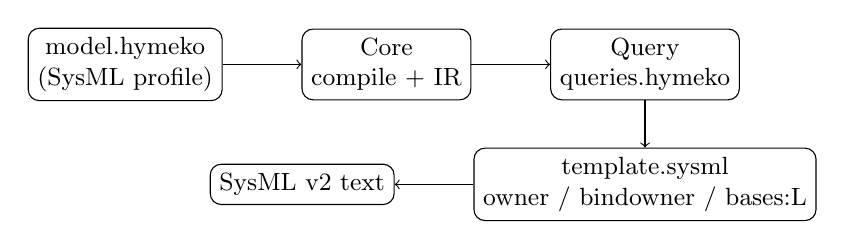
\begin{tikzpicture}[node distance=6mm and 10mm, every node/.style={draw, rounded corners, font=\small, align=center}]
\node (m) {model.hymeko\\(SysML profile)};
\node (c) [right=of m] {Core\\compile + IR};
\node (q) [right=of c] {Query\\queries.hymeko};
\node (t) [below=of q] {template.sysml\\owner / bindowner / bases:L};
\node (o) [left=of t] {SysML v2 text};
\draw[->] (m) -- (c); \draw[->] (c) -- (q); \draw[->] (q) -- (t); \draw[->] (t) -- (o);
\end{tikzpicture}
\end{center}
\end{document}
